\label{sec:results_body}

\subsection{Descriptive evidence}\label{ssec:descriptives}

Across the 100 pre-treatment top tags, weekly question
volume fell from $\sim$44{,}200 pre-ChatGPT to $\sim$15{,}300
post (a $-65.3\%$ change). Substitutable question types fell
$-65.8\%$ versus $-53.4\%$ for non-substitutable types, and
within AI-answerability quartiles the decline is
monotonically larger for higher quartiles (Q1 $-58.5\%$;
Q4 $-67.9\%$). At the tag level the partial correlation
between $\Delta\log(1+Q)$ and the structural answerability
score is $r=-0.38$ ($p<10^{-4}$, $n=100$).

\begin{figure}[!htbp]
\centering
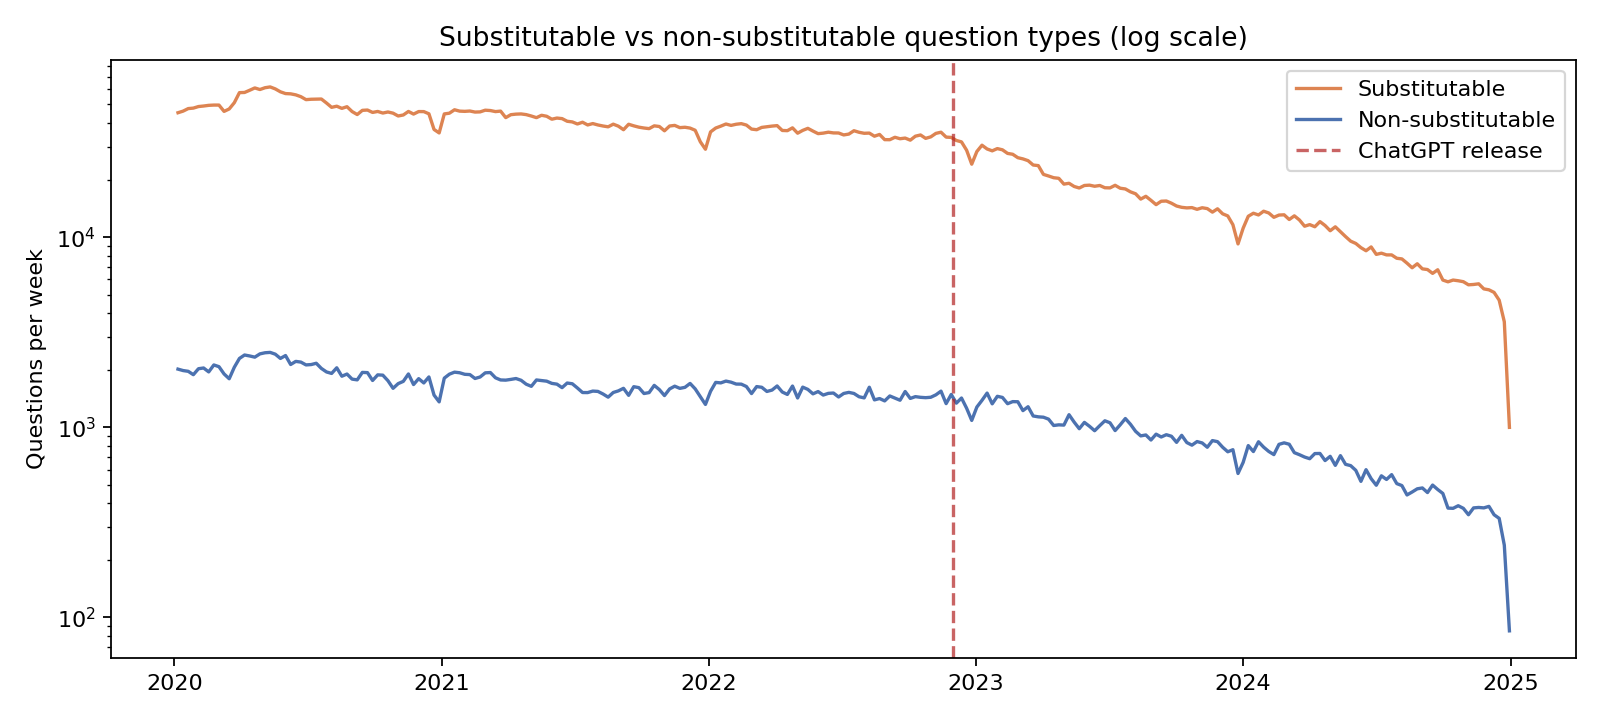
\includegraphics[width=0.82\textwidth]{figures/macro_substitutable_vs_not_log.png}
\caption{Weekly questions by substitutability, 2020--2024 (log
scale). Vertical line: ChatGPT release.}
\label{fig:macro_sub_vs_not}
\end{figure}

\subsection{Baseline DDD coefficient}\label{ssec:main_baseline}

The conservative inclusive baseline---retaining
advanced-architecture questions in the control and using the
full sample with the historical answerability index---is
$\hat\beta_{\text{DDD}}=-0.108$ (CR1 SE $0.046$, $p=0.021$).
Our preferred specification excludes the declared boundary
category advanced-architecture from the control
(\S\ref{ssec:data_ai_answerability}) and gives $-0.140$
($p=0.005$); restricting the substitutability label to the
high-agreement subsample gives $\approx-0.11$. The treatment
is measured two ways: the historical index and a co-primary
embedding-based answerability score that uses \emph{no} Stack
Overflow historical features ($-0.119$, $p<0.001$). The two
measures share none of their inputs, so we read the gradient
as answerability-driven rather than historical popularity,
without overselling their $r\approx0.4$--$0.5$ convergence as
more than moderate. The full robustness battery (alternative
proxies, sub-samples, leave-one-out, PPML, two-way
clustering, wild bootstrap, and a 32-cell specification curve
that is negative and significant in 100\% of cells) is in the
replication package.

\subsection{Support-post funnel}\label{ssec:results_funnel}

Existing displacement studies measure platform activity
(new questions). From a knowledge-production perspective the
relevant outcome is the production of posts that pass
observable support gates: answered, accepted by the asker,
not closed, and non-negative in net score---a
\emph{funnel-qualified post}. The term is deliberately
narrower than durable reuse, which the public data do not
observe; each gate is meaningful because it is operated by a
different actor (answerer, asker, moderator, crowd). We build
a five-transition funnel at the (tag, week, question-type)
cell from the $8{,}404{,}411$-question stream; only $38.0\%$
survive to the funnel-qualified stage. Re-fitting the
baseline DDD with each funnel stage as the outcome
(Table~\ref{tab:reusable_funnel}) gives a relative
coefficient that is stable across stages
($-0.108$ to $-0.121$, all $p<0.05$), so the implied
cumulative shortfall over the 109 post-ChatGPT weeks
contracts from $\sim$70{,}000 missing questions to
$\sim$28{,}000 missing funnel-qualified posts (about $40\%$
of the activity shortfall). The stability is partly
mechanical---the gates are nested---so the funnel is best
read as an operational accounting device from the volume
coefficient to observed support counts, not as evidence on
where in the value distribution the channel falls; that is
the value-weighted question we test next.

\begin{table}[ht]
\centering
\caption{Triple-difference (DDD) estimates across the observed support-post funnel. The dependent variable is $\log(1+Y_{twk})$ where $Y$ is the cell-level count. Coefficients on the triple interaction $\text{AI}_k \cdot \text{Post}_t \cdot \text{Sub}_k$ are reported, with tag-clustered standard errors in parentheses. The implied shortfall is computed as $\sum_{\text{post}}(Y \cdot e^{-\hat\beta \cdot \text{AI} \cdot \text{Sub}} - Y)$.}
\label{tab:reusable_funnel}
\small
\setlength{\tabcolsep}{4pt}
\begin{adjustbox}{max width=\textwidth}
\begin{tabular}{lrrrrrr}
\toprule
Funnel stage & $\hat\beta_{DDD}$ & SE & $p$ & 95\% CI & N obs & Implied shortfall \\
\midrule
Questions & -0.1082 & (0.0460) & 0.0206 & [-0.199, -0.017] & 164,351 & 70,364 \\
Answered & -0.1150 & (0.0463) & 0.0147 & [-0.207, -0.023] & 164,351 & 61,210 \\
Accepted answer & -0.1168 & (0.0476) & 0.0159 & [-0.211, -0.022] & 164,351 & 32,809 \\
Accepted, not closed & -0.1210 & (0.0480) & 0.0134 & [-0.216, -0.026] & 164,351 & 31,836 \\
Accepted, score $\geq 0$ & -0.1154 & (0.0484) & 0.0190 & [-0.211, -0.019] & 164,351 & 28,504 \\
Funnel-qualified post & -0.1183 & (0.0487) & 0.0169 & [-0.215, -0.022] & 164,351 & 28,001 \\
\bottomrule
\end{tabular}
\end{adjustbox}
\end{table}


\subsection{Value-weighted posts: the benign-pruning
test}\label{ssec:results_value_weighted}

The benign-pruning reading of the aggregate contraction
\citep{xue2026chatgpt} predicts that the channel concentrates
on the low-value end: LLMs absorb routine, low-score queries
that public Q\&A would not have retained in any case. We test
this at the within-tag value margin by re-fitting the DDD on
posts cut by crowd-validation score (in the raw stream, $51\%$
of funnel-qualified posts reach score $\geq1$ and only $4\%$
reach score $\geq5$).

\paragraph{A single pre-specified shape test (primary C1).}
To avoid resting the claim on a family of per-threshold tests,
we pre-specify one statistic (Table~\ref{tab:shape_test}):
stacking the six mutually exclusive net-score bins in one
model, we fit the triple difference plus its interaction with
the centred score level. The \emph{average} displacement
across the value distribution is $-0.167$ ($p<10^{-4}$)---a
single, clearly negative coefficient establishing that the
channel is not confined to score-zero posts---and the
\emph{slope} over score is $-0.094$ ($p=2\times10^{-4}$),
quantifying attenuation toward the elite tail. This is our
primary statement of C1.

\begin{table}[ht]
\centering
\caption{Pre-specified shape test of the value gradient. A single model stacks the six mutually exclusive net-score bins and fits the triple difference plus its interaction with the (centred) net-score level, clustered by tag. The \emph{average} coefficient tests whether the displacement is present across the value distribution (the focal C1 hypothesis); the \emph{slope} tests how it varies with score. This replaces multiple per-bin tests with one declared statistic.}
\label{tab:shape_test}
\small
\begin{tabular}{lrr}
\toprule
Quantity & Estimate & $p$ \\
\midrule
Average displacement across bins & -0.167 & 0.000 \\
Slope over net-score level & -0.094 & 0.000 \\
\bottomrule
\end{tabular}
\end{table}

\paragraph{Consistent corroboration.}
The mutually exclusive bins are flat across the low-to-mid
range ($-0.21$, $-0.20$, $-0.21$ at score $0,1,2$) and
attenuate above ($-0.164$, $-0.124$, $-0.091$ at $3,4,\geq5$);
bins $0$ through $4$ are each individually significant at
$p<0.005$ and survive a Bonferroni correction, so the
\emph{strict} benign-pruning hypothesis (displacement confined
to score-zero posts) is rejected by four separately
significant non-zero-score bins. The elite-tail bin
(score $\geq5$, $-0.091$, $p=0.116$) is underpowered
(MDE $0.16$) and we take its raw null at face value. A
conservative Romano--Wolf correction over the \emph{nested
cumulative} thresholds---which folds the underpowered elite
tail into every statistic---places that particular gradient at
the $10\%$ joint level; we report it in the replication
package as a stringent joint lens, not the headline. The
honest reading is therefore the \emph{shape}: displacement is
roughly proportional across the crowd-validated range and
fades only at the elite tail.

\subsection{Dynamics, pre-trends, and
placebos}\label{ssec:dynamics_event}

The quarterly event-study coefficient is negative and
significant in every post-treatment bin, growing
monotonically from $-0.063$ at $T{+}0$ to $-0.544$ at
$T{+}8$ (Q4 2024); pre-period coefficients are smaller (about
a third of the post mean) and converge toward zero as the
cutoff approaches (Figure~\ref{fig:event_study}).

\begin{figure}[!htbp]
\centering
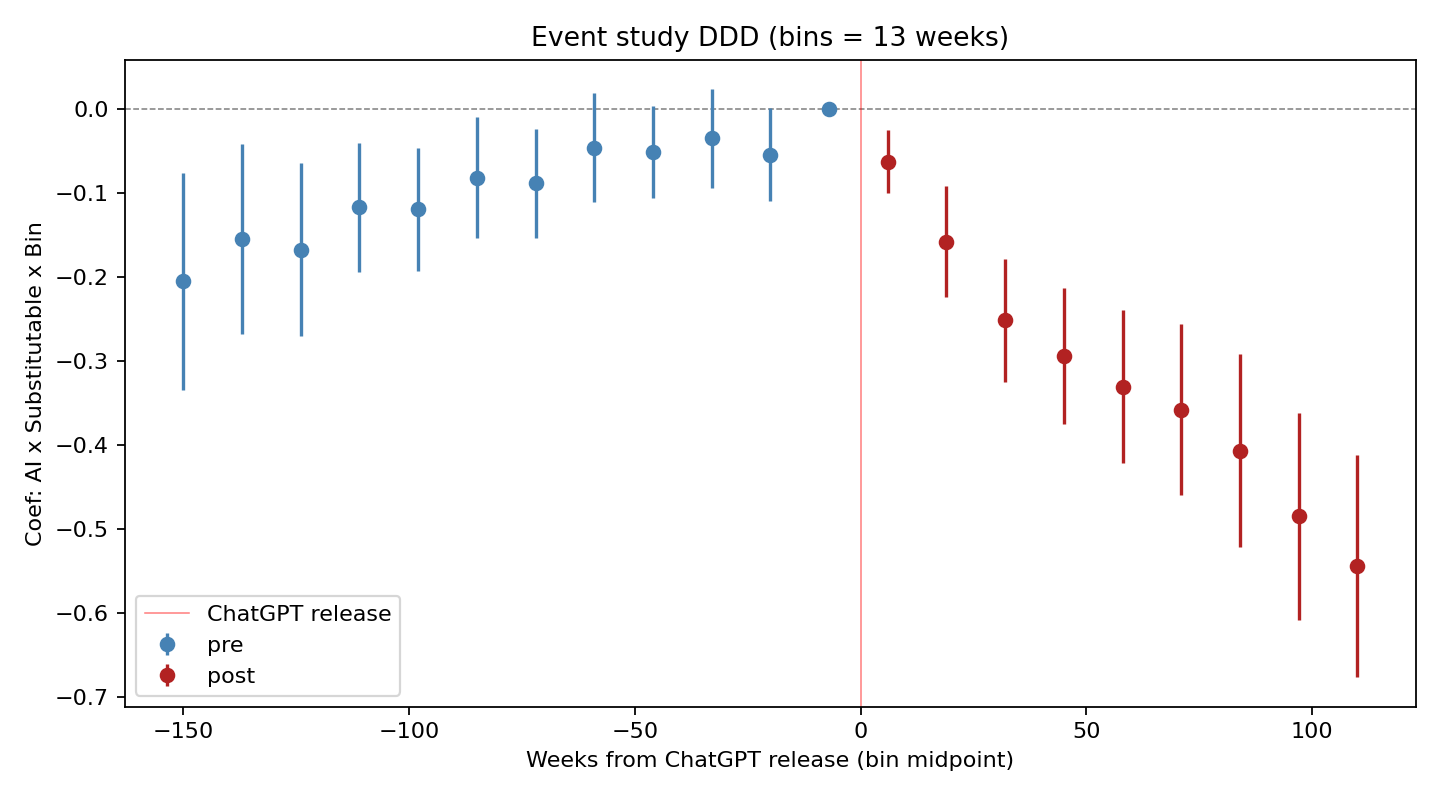
\includegraphics[width=0.82\textwidth]{figures/event_study_ddd_question_type_quarterly.png}
\caption{Quarterly event-study coefficients on
$\text{AI}\times\text{Sub}\times\text{bin}$. Reference: bin
$-1$ (immediately pre-treatment).}
\label{fig:event_study}
\end{figure}

Formal pre-trend tests reject exact parallel trends, so we do
not claim a standalone natural experiment; the estimates are
conditional post-ChatGPT associations whose credibility rests
on a conjunction of diagnostics. Under the official HonestDiD
$\Delta^{\text{RM}}$ implementation the breakdown is
$\bar M = 0.75$ (the robust 95\% CI first contains zero at
$\bar M = 0.75$; it remains $[-0.136,-0.010]$ at
$\bar M = 0.50$), which we read as a moderate signal. Five
conventional pre-period placebos return \emph{positive}
coefficients ($+0.059$ to $+0.067$, all $p<0.012$), and a
29-step rolling-placebo sweep (mean $+0.057$) contains no
cutoff as negative as the real one---a sign reversal hard to
reconcile with a smooth continuation of the pre-period path.
A June 2022 GitHub Copilot placebo is also positive
($+0.058$, $p=0.011$); in a joint model the ChatGPT
interaction is $-0.157$ ($p<0.001$) while Copilot stays
$+0.058$. Full event-study, placebo, and specification-curve
detail is in the replication package.

\subsection{Magnitude}\label{ssec:magnitude}\label{ssec:magnitude_benchmarks}

Applying the coefficient cell-by-cell to the post-period
panel implies $\sim$70{,}000 missing questions over the 109
post-ChatGPT weeks---$4.2\%$ of the $1{,}671{,}197$ observed
post-period questions in the top-100-tag panel. The implied
displaced high-value (score $\geq1$) flow is $\sim$15{,}200
posts ($0.9\%$ of all observed questions). Whether this small
flow matters is a stock--flow question: the public archive is
a durable stock, so a persistent reduction in the high-value
\emph{flow} ($\sim$7{,}300 posts/year at the window average)
accumulates to $\sim$36{,}000 over five years under a constant
flow. We present these as transparent projections under stated
assumptions, not forecasts, and they do not bear on welfare or
generalise beyond the panel. Benchmarked against a descriptive
linear extrapolation of the pre-trend ($\sim$1.42 million
questions), the DDD-estimated channel is about $5\%$---a
\emph{discipline} on causal interpretation: the aggregate
decline cannot all be attributed to LLM substitutability
without further identification.
